
\section{Model Predictive Control}

\begin{frame}[t]
	\frametitle{Learning Problem}
	
	\vspace{-0.75cm}
	%    \setbeamercovered{transparent}
	
	\begin{columns}[t]
		
		\begin{column}{0.33\textwidth}
			%	  \begin{tcolorbox}{}	  
			%	  \end{tcolorbox} 	
			\begin{center}
				\Large
				\textcolor{mycolor}{weather} \\
				\small
				\vspace{0.4cm}
				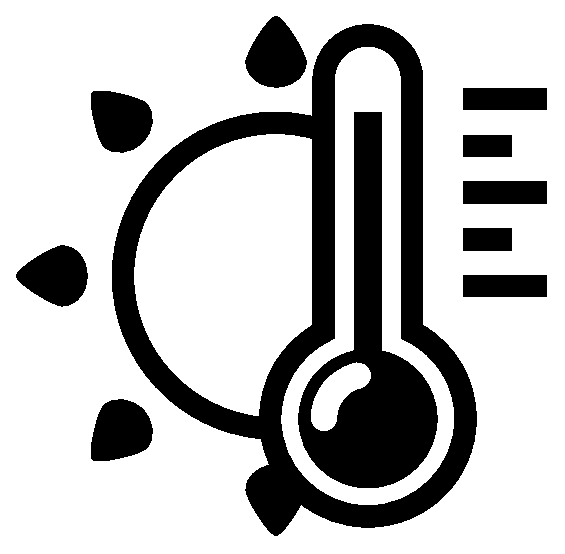
\includegraphics[width=3pc]{figures/temperature.eps}\\
				\begin{itemize}
					%					\centering
					\item \color{red} outside temp. $\tX^{d_1}$
					\item outside humidity $\tX^{d_2}$
					\item solar radiation $\tX^{d_3}$
				\end{itemize}
			\end{center}
		\end{column}
		
		\begin{column}{0.33\textwidth}
			\begin{center}
				\Large
				\textcolor{mycolor}{building} \\
				\small
				\vspace{0.4cm}
				\includegraphics[width=3pc]{figures/building.eps}
				\begin{itemize}
					\centering
					\item \color{blue} power consumption $\tY$
					\item \color{red} internal gains $\tX^{d_4}$
					
				\end{itemize}
			\end{center}
		\end{column}
		
		\begin{column}{0.33\textwidth}
			\begin{center}
				\Large
				\textcolor{mycolor}{control} \\
				\small
				\vspace{0.4cm}
				\includegraphics[width=3pc]{figures/controls.eps}
			\end{center}
			\begin{center}
				\begin{itemize}
					\centering
					\item \color{ForestGreen} cooling temp. $\tX^{c_1}$
					\item \color{ForestGreen} supply air temp. $\tX^{c_2}$
					\item \color{ForestGreen} chilled water temp. $\tX^{c_3}$
				\end{itemize}
			\end{center}
		\end{column}
		
	\end{columns}
	
	\vspace{0.5cm}
	
	The goal is to predict the zone temperature for multiple steps ahead
	\begin{gather*}
	\begin{pmatrix}
	\color{blue} \tY_{\mathrm{k+1}} \\
	\color{blue} \tY_{\mathrm{k+2}} \\
	\color{blue} \vdots \\
	\color{blue} \tY_{\mathrm{k+N}}
	\end{pmatrix}
	= \mathit{f} ( \overbrace{\color{red} \underbrace{\tX^{d}_{k}, \dots, \tX^{d}_{k+N-1}}_\text{disturbance} \color{black},\color{blue} \underbrace{\tY_{\mathrm{k}},\dots, \tY_{\mathrm{k-\delta}}}_\text{autoregression}}^\text{non-manipulated variables}
	\color{black} ,\overbrace{
		\color{ForestGreen} \tX^{c}_{k}, \dots, \tX^{c}_{k+N-1}}^\text{control variables} \color{black})
	\end{gather*}
	
	
\end{frame}


\begin{frame}[t]
	
	\frametitle{Blackbox models}
	
	\begin{gather*}
	\color[RGB]{190,81,8} y_t = \color{black}\mathit{f} (\overbrace{\color[RGB]{190,81,8} \underbrace{y_{t-l}, \dots, y_{t-1}}_\text{autoregression}, \color[RGB]{29,73,153} \underbrace{ w_{t-m}, \dots, w_t}_\text{disturbance} \color{black}}^\text{non-manipulated variables}
	\color{black} ,\overbrace{\color[RGB]{74,133,34} u_{t-p}, \dots, u_t}^\text{control variables} \color{black})
	\end{gather*}
	
	\begin{align*}
	y_t = f(y_{t-l}, \dots, y_{t-1}, w_{t-m}, \dots, w_t, u_{t-p}, \dots, u_t)
	\end{align*}
	
\end{frame}

\begin{frame}[t]
	
	\frametitle{Blackbox models}
	
	\begin{align*}
	P_t = f_P(P_{t-l}, \dots, P_{t-1}, w_{t-m}, \dots, w_{t}, u_{t-p}, \dots, u_{t})
	\end{align*}
	
	\begin{align*}
	T_t^i & = f_T^i(T_{t-l'}, \dots, T_{t-1}, w_{t-m'}, \dots, w_{t}, u_{t-p'}, \dots, u_{t}) \\
	i  & \in \{ 1, \dots, \text{number of zones} \}
	\end{align*}
	
	\begin{align*}
	&\minimize_{u_t,\dots,u_{N-1}} \  \  \sum_{t=0}^{N-1} (P_{t}\!-\!P_{\mathrm{ref}})^2\\
	& 
	\begin{aligned}
	\subjectto \  \  & P_t = f_P(P_{t-l}, \dots, P_{t-1}, w_{t-m}, \dots, w_{t}, u_{t-p}, \dots, u_{t}) \\
	& T_t^i = f_T^i(T^i_{t-l'}, \dots, T^i_{t-1}, w_{t-m'}, \dots, w_{t}, u_{t-p'}, \dots, u_{t}) \\
	& T_{\mathrm{min}} \leq T_{t}^i \leq T_{\mathrm{max}} \\	
	& u_{\mathrm{min}} \leq u_{t} \leq u_{\mathrm{max}} \\
	& t \in \{ 0, \dots, N-1 \}
	\end{aligned}
	\end{align*}
	
\end{frame}


\begin{frame}[t]
	
	\frametitle{Why can't we use black-box models for control?}
	
		\begin{gather*}
		\color[RGB]{190,81,8} P_t = \color{black}\mathit{f} (\overbrace{\color[RGB]{190,81,8} \underbrace{P_{t-l}, \dots, P_{t-1}}_\text{autoregression}, \color[RGB]{29,73,153} \underbrace{ w_{t-m}, \dots, w_t}_\text{disturbance} \color{black}}^\text{non-manipulated variables}
		\color{black} ,\overbrace{\color[RGB]{74,133,34} u_{t-p}, \dots, u_t}^\text{control variables} \color{black}) \\
		\forall t =1,\dots, N.
		\end{gather*}
		
		\begin{align*}
		&\minimize_{u_t,\dots,u_{N-1}} \  \  \sum_{t=0}^{N-1} (P_{t}\!-\!P_{\mathrm{ref}})^2\\
		& 
		\begin{aligned}
		\subjectto \  \  & \color[RGB]{190,81,8} P_t = \color{red}f_P \color{black} (\color[RGB]{190,81,8} P_{t-l}, \dots, P_{t-1}, \color[RGB]{29,73,153} w_{t-m}, \dots, w_t\color{black}
		\color{black} ,\color[RGB]{74,133,34} u_{t-p}, \dots, u_t \color{black}) \\
		 & \color[RGB]{190,81,8} T_t^i  =  \color{red}f_T \color{black} (\color[RGB]{190,81,8} T^i _{t-l'}, \dots, T^i_{t-1}, \color[RGB]{29,73,153} w_{t-m'}, \dots, w_t\color{black} \color{black} ,\color[RGB]{74,133,34} u_{t-p'}, \dots, u_t \color{black}) \\
		& T_{\mathrm{min}} \leq T_{t}^i \leq T_{\mathrm{max}} \\	
		& u_{\mathrm{min}} \leq u_{t} \leq u_{\mathrm{max}} \\
		& t \in \{ 0, \dots, N-1 \}
		\end{aligned}
		\end{align*}
	
\end{frame}

\begin{frame}[t]
	
	\frametitle{Model Predictive Control}
	
%	\color{blue} Prediction with \textit{zero-variance method} \color{black}
%	
%	\begin{align*}
%		y_{t+\tau} &\sim \GaussianDist{\bar{y}_{t+\tau}}{\sigma^2_{y,t+\tau}} \\
%		\bar{y}_{t+\tau} &= \mu(x_{t+\tau}) + K_\star K^{-1} (Y - \mu(X)) \\
%		\sigma^2_{y,t+\tau} &= K_{\star \star} - K_\star K^{-1} K_\star^T \\
%		K_\star &= [k(x_{t+\tau}, x_1), \dots, k(x_{t+\tau}, x_N)], K_{\star \star} = k(x_{t+\tau}, x_{t+\tau}) \\
%		x_{t + \tau} &= [\bar y_{t+ \tau-l}, \dots, \bar y_{t+ \tau-1}, u_{t+ \tau-m}, \dots, u_{t+ \tau}, w_{t+ \tau-p}, \dots, w_{t+ \tau-1}, w_{t+ \tau}]
%	\end{align*}
	
	\begin{align*}
	&\minimize_{u_t,\dots,u_{N-1}} \  \  \sum_{\tau=0}^{N-1} (\bar{P}_{t+\tau}\!-\!P_{\mathrm{ref}})^2 \color{red} \!+\! \lambda \sigma^2_{P,t+\tau}\\
	&
	\begin{aligned}
	\subjectto \  \  
	&  \color[RGB]{29,73,153} \begin{rcases}
	 \color[RGB]{29,73,153} \bar{P}_{t+\tau} = \mu(x_{t+\tau}) + K_\star K^{-1} (Y - \mu(X)) \nonumber\\
	 \color[RGB]{29,73,153} \sigma^2_{P,t+\tau} = K_{\star \star} - K_\star K^{-1} K_\star^T
	\end{rcases}  \color[RGB]{29,73,153} \text{power model}\\
	& \color[RGB]{74,133,34} \begin{rcases}
	\color[RGB]{74,133,34} \bar{T}_{t+\tau} = \mu(x_{t+\tau}) + K_\star K^{-1} (Y - \mu(X)) \nonumber\\
	\color[RGB]{74,133,34} \sigma^2_{T,t+\tau} = K_{\star \star} - K_\star K^{-1} K_\star^T
	\end{rcases} \color[RGB]{74,133,34} \text{temperature model}\\
	& u_{\mathrm{min}} \leq u_{t+\tau} \leq u_{\mathrm{max}} \\
	& \tau \in \{ 0, \dots, N-1 \} \\
	& \color{red} \Pr(T_{\mathrm{min}} \leq T_{t+\tau} \leq T_{\mathrm{max}}) \geq 1 - \epsilon \nonumber
	\end{aligned}
\end{align*}

\end{frame}

\begin{frame}[t]
	
	\frametitle{Data-driven MPC}
	
	\begin{align*}
	&\minimize_{u_t,\dots,u_{N-1}} \  \  \sum_{\tau=0}^{N-1} (\bar{P}_{t+\tau}\!-\!P_{\mathrm{ref}})^2 \color{red} \!+\! \lambda \sigma^2_{P,t+\tau}\\
	&
	\begin{aligned}
	\subjectto \  \  
	&  \color{red} \begin{rcases}
	\color{red} \bar{P}_{t+\tau} = \mu(x_{t+\tau}) + K_\star K^{-1} (Y - \mu(X)) \nonumber\\
	\color{red} \sigma^2_{P,t+\tau} = K_{\star \star} - K_\star K^{-1} K_\star^T
	\end{rcases}  \color{red} \text{power model}\\
	& \color{red} \begin{rcases}
	\color{red} \bar{T}_{t+\tau} = \mu(x_{t+\tau}) + K_\star K^{-1} (Y - \mu(X)) \nonumber\\
	\color{red} \sigma^2_{T,t+\tau} = K_{\star \star} - K_\star K^{-1} K_\star^T
	\end{rcases} \color{red} \text{temperature model}\\
	& \color{blue} \Pr(T_{\mathrm{min}} \leq T_{t+\tau} \leq T_{\mathrm{max}}) \geq 1 - \epsilon \\	
	& u_{\mathrm{min}} \leq u_{t+\tau} \leq u_{\mathrm{max}} \\
	& \tau \in \{ 0, \dots, N-1 \}
	\end{aligned}
	\end{align*}
	
\end{frame}

\begin{frame}[t]
	
	\frametitle{Physics-based MPC}
	
	\begin{align*}
	&\minimize_{u_t,\dots,u_{N-1}} \  \  \sum_{\tau=0}^{N-1} (P_{t+\tau}(x_{t+\tau})\!-\!P_{\mathrm{ref}})^2 \color{red} \\
	&
	\begin{aligned}
	\subjectto \  \  
	& \color{red}x_{t+\tau} =  Ax_{t+\tau-1} + B u_{t+\tau-1} + B_w w_{t+\tau-1} \\
	& \color{red}B = B_u + B_{xu}[x_{t+\tau-1}] + B_{wu}[w_{t+\tau-1}] \\
	& \color{blue} T_{\mathrm{min}} \leq T_{t+\tau}(x_{t+\tau}) \leq T_{\mathrm{max}} \\	
	& u_{\mathrm{min}} \leq u_{t+\tau} \leq u_{\mathrm{max}} \\
	& \tau \in \{ 0, \dots, N-1 \}
	\end{aligned}
	\end{align*}
	
\end{frame}

\begin{frame}[t]
	
	\frametitle{OED Example}
	\begin{figure}[t]
		\centering
		\setlength\fwidth{0.9\textwidth}
		\setlength\hwidth{0.3\textwidth}
		% This file was created by matlab2tikz.
%
%The latest updates can be retrieved from
%  http://www.mathworks.com/matlabcentral/fileexchange/22022-matlab2tikz-matlab2tikz
%where you can also make suggestions and rate matlab2tikz.
%
\definecolor{mycolor1}{rgb}{0.00000,0.44700,0.74100}%
\definecolor{mycolor2}{rgb}{0.49400,0.18400,0.55600}%
\definecolor{mycolor3}{rgb}{0.85000,0.32500,0.09800}%
\definecolor{mycolor4}{rgb}{0.46600,0.67400,0.18800}%
%
\begin{tikzpicture}

\begin{axis}[%
width=\fwidth,
height=0.972\hwidth,
at={(0\fwidth,0\hwidth)},
scale only axis,
unbounded coords=jump,
xmin=28,
xmax=80,
xtick={40,52,56,64,68},
xticklabels={{10am},{1pm},{2pm},{4pm},{5pm}},
ymin=0.9,
ymax=1.4,
ylabel style={font=\color{white!15!black}},
ylabel={power [MW]},
axis background/.style={fill=white},
xmajorgrids,
ymajorgrids,
legend style={at={(0.5,1.03)}, anchor=south, legend columns=4, legend cell align=left, align=left, fill=none, draw=none},
xlabel style={font=\normalsize},ylabel style={font=\normalsize},legend style={font=\normalsize},ticklabel style={font=\normalsize},ylabel shift = -5 pt,xlabel shift = -5 pt,
]
%\addplot [color=mycolor1, line width=0.8pt]
%  table[row sep=crcr]{%
%28	0.701337270215983\\
%29	0.964386864105802\\
%30	1.07611937785975\\
%31	1.07965889013915\\
%32	1.08263425777965\\
%33	1.0487078852313\\
%34	1.36010806924978\\
%35	1.36759900325363\\
%36	1.36760719930364\\
%37	1.32098352764474\\
%38	1.32242976345489\\
%39	1.32380671627597\\
%40	1.32514010664879\\
%41	1.32924061035125\\
%42	1.30938781215828\\
%43	1.31134364830977\\
%44	1.31188016501142\\
%45	1.2500852134782\\
%46	1.24646728713905\\
%47	1.24503606638487\\
%48	1.24284947538557\\
%49	1.3054168397276\\
%50	1.31084852897669\\
%51	1.31383043363787\\
%52	1.31722883499294\\
%53	1.25655812988594\\
%54	1.25098658270947\\
%55	1.2463345049663\\
%56	1.22752780626403\\
%57	1.2208541993049\\
%58	1.22128329266941\\
%59	1.20413855244015\\
%60	1.21065177839894\\
%61	1.27896217800335\\
%62	1.2605057789187\\
%63	1.25372092775248\\
%64	1.25124511806312\\
%65	1.31403271159904\\
%66	1.35557591722558\\
%67	1.37171201603009\\
%68	1.36365154437866\\
%69	1.29437500894808\\
%70	1.19254042423185\\
%71	1.18622722392824\\
%72	1.18074059232931\\
%73	1.14206208162902\\
%74	1.02430601488298\\
%75	1.00838459412059\\
%76	0.994868730990595\\
%77	0.930693792044902\\
%78	0.972997064435496\\
%79	0.966290070561223\\
%80	0.960576891269175\\
%};
%\addlegendentry{system}

\addplot [color=mycolor2, line width=0.8pt]
  table[row sep=crcr]{%
28	0.698656568402034\\
29	0.960110193762699\\
30	1.07117661302724\\
31	1.07450227005384\\
32	1.07751590209242\\
33	1.04361693743596\\
34	1.35436168467098\\
35	1.36154860058372\\
36	1.3617333326939\\
37	1.31517558533323\\
38	1.31674255055187\\
39	1.31825553821012\\
40	1.31973188294945\\
41	1.32388058858893\\
42	1.3050436135893\\
43	1.30704312156872\\
44	1.30766610755565\\
45	1.24638537676761\\
46	1.24300968498255\\
47	1.24168296642299\\
48	1.23962397881658\\
49	1.30186627149222\\
50	1.30721893878346\\
51	1.31024436270579\\
52	1.31364780877709\\
53	1.31384445792102\\
54	1.31240928835398\\
55	1.30997587797896\\
56	1.30686708508127\\
57	1.30417518875771\\
58	1.30171225137563\\
59	1.29966621173883\\
60	1.29789136564455\\
61	1.34644408799804\\
62	1.34695403514791\\
63	1.34754008400916\\
64	1.34980467811679\\
65	1.33078629098477\\
66	1.3579711076543\\
67	1.3608334854345\\
68	1.3671692932846\\
69	1.25615299231862\\
70	1.14823562129838\\
71	1.14520812110636\\
72	1.14387262675201\\
73	1.11057462575508\\
74	0.998293109136584\\
75	0.986840963134787\\
76	0.976546372495654\\
77	0.91559944312747\\
78	0.96002086329302\\
79	0.954769359624132\\
80	0.95025187381431\\
};
\addlegendentry{baseline}

%\addplot [color=mycolor3, line width=0.8pt]
%  table[row sep=crcr]{%
%28	0.730190371183039\\
%29	0.722429385563428\\
%30	1.06112688842685\\
%31	1.10442088033856\\
%32	1.11097058774604\\
%33	1.07174659396359\\
%34	1.32580637819376\\
%35	1.34973144914331\\
%36	1.3382219987633\\
%37	1.30591030816251\\
%38	1.27642888607857\\
%39	1.28270243657784\\
%40	1.27904428148941\\
%41	1.29895660528902\\
%42	1.28547646010141\\
%43	1.28353259843374\\
%44	1.29018858651565\\
%45	1.2889386593834\\
%46	1.27556383097544\\
%47	1.26307241028446\\
%48	1.25677225354276\\
%49	1.23884924304318\\
%50	1.30616384842031\\
%51	1.31999607713492\\
%52	1.32858703257795\\
%53	1.26733226726688\\
%54	1.24933166543075\\
%55	1.24128592735231\\
%56	1.2169295806082\\
%57	1.21422291514978\\
%58	1.21172261139135\\
%59	1.20973623510218\\
%60	1.20795392025831\\
%61	1.25642645485439\\
%62	1.25692084314693\\
%63	1.25747268111749\\
%64	1.25976227623582\\
%65	1.3307068647466\\
%66	1.35794619649566\\
%67	1.36080393869416\\
%68	1.36714147767466\\
%69	1.38994755537238\\
%70	1.20344445838934\\
%71	1.17162583164319\\
%72	1.14798368704629\\
%73	1.1554174858564\\
%74	1.03296169058873\\
%75	1.00545391405229\\
%76	0.995942240487405\\
%77	0.972458103570065\\
%78	0.915100501572983\\
%79	0.966356316537056\\
%80	0.946162514908633\\
%};
%\addlegendentry{$\mu$}

%\addplot [color=mycolor4, dashed, line width=0.8pt]
%  table[row sep=crcr]{%
%28	nan\\
%29	nan\\
%30	nan\\
%31	nan\\
%32	nan\\
%33	nan\\
%34	nan\\
%35	nan\\
%36	nan\\
%37	nan\\
%38	nan\\
%39	nan\\
%40	nan\\
%41	nan\\
%42	nan\\
%43	nan\\
%44	nan\\
%45	nan\\
%46	nan\\
%47	nan\\
%48	nan\\
%49	nan\\
%50	nan\\
%51	nan\\
%52	nan\\
%53	nan\\
%54	nan\\
%55	nan\\
%56	1.21686708508127\\
%57	1.21417518875771\\
%58	1.21171225137563\\
%59	1.20966621173883\\
%60	1.20789136564455\\
%61	1.25644408799804\\
%62	1.25695403514791\\
%63	1.25754008400916\\
%64	1.25980467811679\\
%65	1.33078629098477\\
%66	1.3579711076543\\
%67	1.3608334854345\\
%68	1.3671692932846\\
%69	nan\\
%70	nan\\
%71	nan\\
%72	nan\\
%73	nan\\
%74	nan\\
%75	nan\\
%76	nan\\
%77	nan\\
%78	nan\\
%79	nan\\
%80	nan\\
%};
%\addlegendentry{reference}

\addplot [color=black, dashed, line width=0.8pt, forget plot]
  table[row sep=crcr]{%
52	0\\
52	5.55555555555556\\
52	11.1111111111111\\
52	16.6666666666667\\
52	22.2222222222222\\
52	27.7777777777778\\
52	33.3333333333333\\
52	38.8888888888889\\
52	44.4444444444444\\
52	50\\
};
\addplot [color=black, dashed, line width=0.8pt, forget plot]
  table[row sep=crcr]{%
56	0\\
56	5.55555555555556\\
56	11.1111111111111\\
56	16.6666666666667\\
56	22.2222222222222\\
56	27.7777777777778\\
56	33.3333333333333\\
56	38.8888888888889\\
56	44.4444444444444\\
56	50\\
};
\addplot [color=black, dashed, line width=0.8pt, forget plot]
  table[row sep=crcr]{%
64	0\\
64	5.55555555555556\\
64	11.1111111111111\\
64	16.6666666666667\\
64	22.2222222222222\\
64	27.7777777777778\\
64	33.3333333333333\\
64	38.8888888888889\\
64	44.4444444444444\\
64	50\\
};
\addplot [color=black, dashed, line width=0.8pt, forget plot]
  table[row sep=crcr]{%
68	0\\
68	5.55555555555556\\
68	11.1111111111111\\
68	16.6666666666667\\
68	22.2222222222222\\
68	27.7777777777778\\
68	33.3333333333333\\
68	38.8888888888889\\
68	44.4444444444444\\
68	50\\
};
\end{axis}
\end{tikzpicture}%
	\end{figure}
	
\end{frame}

\begin{frame}[t]
	
	\frametitle{OED Example}
	\begin{figure}[t]
		\centering
		\setlength\fwidth{0.9\textwidth}
		\setlength\hwidth{0.3\textwidth}
		\input{figures/control-tracking-reference.tex}
	\end{figure}
	
\end{frame}

\begin{frame}[t]
	
	\frametitle{OED Example}
	\begin{figure}[t]
		\centering
		\setlength\fwidth{0.9\textwidth}
		\setlength\hwidth{0.3\textwidth}
		\input{figures/control-tracking-system.tex}
	\end{figure}
	
\end{frame}

%\begin{frame}[t]
%	
%	\frametitle{OED Example}
%	\begin{figure}[t]
%		\centering
%		\setlength\fwidth{0.9\textwidth}
%		\setlength\hwidth{0.3\textwidth}
%		\input{figures/control-tracking.tex}
%	\end{figure}
%	
%\end{frame}

\begin{frame}[t]
	
	\frametitle{OED Example}
	\begin{figure}[t]
		\centering
		\setlength\fwidth{0.9\textwidth}
		\setlength\hwidth{0.3\textwidth}
		% This file was created by matlab2tikz.
%
%The latest updates can be retrieved from
%  http://www.mathworks.com/matlabcentral/fileexchange/22022-matlab2tikz-matlab2tikz
%where you can also make suggestions and rate matlab2tikz.
%
\definecolor{mycolor1}{rgb}{0.97647,0.89804,1.00000}%
\definecolor{mycolor2}{rgb}{0.85000,0.32500,0.09800}%
%
\begin{tikzpicture}

\begin{axis}[%
width=0.951\fwidth,
height=\hwidth,
at={(0\fwidth,0\hwidth)},
scale only axis,
unbounded coords=jump,
xmin=28,
xmax=80,
xtick={40,52,56,64,68},
xticklabels={{10am},{1pm},{2pm},{4pm},{5pm}},
ymin=0,
ymax=150,
ylabel style={font=\color{white!15!black}},
ylabel={error [kW]},
axis background/.style={fill=white},
xmajorgrids,
ymajorgrids,
legend style={at={(0.5,0.97)}, anchor=north, legend columns=2, legend cell align=left, align=left, draw=white},
xlabel style={font=\footnotesize},ylabel style={font=\footnotesize},legend style={font=\footnotesize},ticklabel style={font=\footnotesize},ylabel shift = -5 pt,xlabel shift = -5 pt,
]

\addplot[area legend, draw=mycolor1, fill=mycolor1]
table[row sep=crcr] {%
x	y\\
28	97.6098920017012\\
29	87.0616094836532\\
30	111.133048508513\\
31	110.827159840066\\
32	113.977820092415\\
33	101.432643090638\\
34	116.764197799347\\
35	138.144394491007\\
36	131.003515767036\\
37	118.671301193402\\
38	93.1968936559279\\
39	93.0031230408833\\
40	85.9626603158963\\
41	95.1984454575204\\
42	94.470571016182\\
43	89.2501967117046\\
44	89.2640234573722\\
45	87.9949534522782\\
46	85.0583216254288\\
47	90.7399998693282\\
48	98.6742717459474\\
49	86.6002727932765\\
50	89.5009090083115\\
51	86.297390401661\\
52	84.8458696695925\\
53	85.7598494186104\\
54	82.7837124089043\\
55	80.2021271583231\\
56	80.4049505550647\\
57	86.5603710203912\\
58	85.9001968539745\\
59	90.426668177048\\
60	90.5529314299456\\
61	86.881133558221\\
62	90.9749172106499\\
63	85.8906819304997\\
64	81.1619532380134\\
65	79.327344026635\\
66	85.7068812428649\\
67	85.6081513087749\\
68	92.4794687869323\\
69	92.5422429183118\\
70	112.126042020991\\
71	94.7308409901038\\
72	89.8109566961293\\
73	97.4819064918549\\
74	96.354998087439\\
75	105.679970273324\\
76	91.025910924969\\
77	88.5299233517882\\
78	90.5401321803905\\
79	94.2144975581434\\
80	94.0620329496377\\
80	0\\
79	0\\
78	0\\
77	0\\
76	0\\
75	0\\
74	0\\
73	0\\
72	0\\
71	0\\
70	0\\
69	0\\
68	0\\
67	0\\
66	0\\
65	0\\
64	0\\
63	0\\
62	0\\
61	0\\
60	0\\
59	0\\
58	0\\
57	0\\
56	0\\
55	0\\
54	0\\
53	0\\
52	0\\
51	0\\
50	0\\
49	0\\
48	0\\
47	0\\
46	0\\
45	0\\
44	0\\
43	0\\
42	0\\
41	0\\
40	0\\
39	0\\
38	0\\
37	0\\
36	0\\
35	0\\
34	0\\
33	0\\
32	0\\
31	0\\
30	0\\
29	0\\
28	0\\
}--cycle;
\addlegendentry{$\text{2}\sigma$}

\addplot [color=mycolor2, line width=0.8pt]
  table[row sep=crcr]{%
28	nan\\
29	nan\\
30	nan\\
31	nan\\
32	nan\\
33	nan\\
34	nan\\
35	nan\\
36	nan\\
37	nan\\
38	nan\\
39	nan\\
40	nan\\
41	nan\\
42	nan\\
43	nan\\
44	nan\\
45	nan\\
46	nan\\
47	nan\\
48	nan\\
49	nan\\
50	nan\\
51	nan\\
52	11.3581975850125\\
53	10.7741373809408\\
54	1.65491727871677\\
55	5.04857761399467\\
56	10.598225655827\\
57	6.6312841551171\\
58	9.56068127806475\\
59	5.59768266202741\\
60	2.69785814063016\\
61	22.53572314896\\
62	3.58493577176932\\
63	3.7517533650132\\
64	8.51715817269633\\
65	16.6741531475573\\
66	2.37027927008285\\
67	10.9080773359292\\
68	3.48993329599693\\
69	nan\\
70	nan\\
71	nan\\
72	nan\\
73	nan\\
74	nan\\
75	nan\\
76	nan\\
77	nan\\
78	nan\\
79	nan\\
80	nan\\
};
\addlegendentry{prediction error}

\addplot [color=black, dashed, line width=0.8pt, forget plot]
  table[row sep=crcr]{%
52	0\\
52	16.6666666666667\\
52	33.3333333333333\\
52	50\\
52	66.6666666666667\\
52	83.3333333333333\\
52	100\\
52	116.666666666667\\
52	133.333333333333\\
52	150\\
};
\addplot [color=black, dashed, line width=0.8pt, forget plot]
  table[row sep=crcr]{%
56	0\\
56	16.6666666666667\\
56	33.3333333333333\\
56	50\\
56	66.6666666666667\\
56	83.3333333333333\\
56	100\\
56	116.666666666667\\
56	133.333333333333\\
56	150\\
};
\addplot [color=black, dashed, line width=0.8pt, forget plot]
  table[row sep=crcr]{%
64	0\\
64	16.6666666666667\\
64	33.3333333333333\\
64	50\\
64	66.6666666666667\\
64	83.3333333333333\\
64	100\\
64	116.666666666667\\
64	133.333333333333\\
64	150\\
};
\addplot [color=black, dashed, line width=0.8pt, forget plot]
  table[row sep=crcr]{%
68	0\\
68	16.6666666666667\\
68	33.3333333333333\\
68	50\\
68	66.6666666666667\\
68	83.3333333333333\\
68	100\\
68	116.666666666667\\
68	133.333333333333\\
68	150\\
};
\end{axis}
\end{tikzpicture}%
	\end{figure}
	
\end{frame}